%
% teil1.tex -- Beispiel-File für das Paper
%
% (c) 2020 Prof Dr Andreas Müller, Hochschule Rapperswil
%
% !TEX root = ../../buch.tex
% !TEX encoding = UTF-8
%
\section{Unschärferelation
\label{sonogramm:section:teil1}}
\rhead{Unschärferelation}
Wie bereits in der Einleitung des Kapitels angedeutet sind die zusätzlichen
Zeitlichen Informationen nicht gratis. 
Mit dem aufteilen des Ursprünglichen Signals in kurze Fenster bekommen wir eine
verbesserte zeitliche Auflösung, wir verlieren jedoch an Frequenzauflösung.
Zusätzlich werden durch das abrupte abschneiden des Signals mit dem Rechtecksfenster
zusätzliche Frequenzen hinzugefügt. 
Diese Effekte hängen mit der Unschärferelation zusammen, welche in Abschnitt
\ref{buch:diskret:section:unschaerfe} genauer beschrieben ist.
%Dieser Effekt ist auch als "Frequency Leakage" bekannt.
In diesem Abschnitt werden wir diese Effekte genauer untersuchen.
\subsection{Auswirkung der Fensterfunktion}
Der Faltungssatz beschreibt 
\begin{align}
    f(t) * g(t)& \xrightarrow{\mathscr{F}} F(f)G(f),\\
    f(t) g(t)&\xrightarrow{\mathscr{F}}F(f) * G(f).
\end{align}
Das bedeutet, das die Verwendung von Fensterfunktionen das Frequenzspektrum
des Signals mit dem Frequenzspektrum der Fensterfunktion gefaltet wird.
Die Fouriertransformation eines Rechteckfensters ist 
\begin{equation}
    W_r(f) = \frac{\sin(2 \ pi f  L_w / (2 f_s))}{\sin(2 \pi f / (2 f_s))} e^{-i 2 \pi f (L_w-1)/(2f_s)}
\end{equation}
mit $f_s$ als Abtastfrequenz.
Ein Beispiel mit eines Rechteckfensters mit $L_w = 20$ und $f_s = 20$ Hz ist in Abbildung \ref{sonogramm:recttime}
zu sehen.
Das Dazugehörige Frequenzspektrum zeigt Abbildung \ref{sonogramm:rectfreq}. 
Der grosse Peak in der Mitte kommt vom hohen DC Anteil von $w_r$. 
Da wir aber einen Sprung von 0 auf 1 bei $n = 10$ haben und bei $n = 30$ wieder von 
1 auf 0 springen kommen neue Frequenzen dazu. 
Wird nun das Signal mit dem Fenster multipliziert, kommen diese sogenannten Leck-Frequenzen
in das Frequenzspektrum des Signals.


In diesem ist der 
Die Maximale Frequenzauflösung, welche man mit der diskreten Fouriertransformation DTFT erreichen
kann, ist 
\begin{equation}
    \Delta f = \frac{1}{T}
\end{equation}
wobei $T$ die Messzeit des Signales ist.


% \begin{figure}
%     \centering
%     \subfigure[Rechtecksfenster mit $L_w = 20$ und T = 1 Sekunde. \label{sonogramm:recttime}]
%       {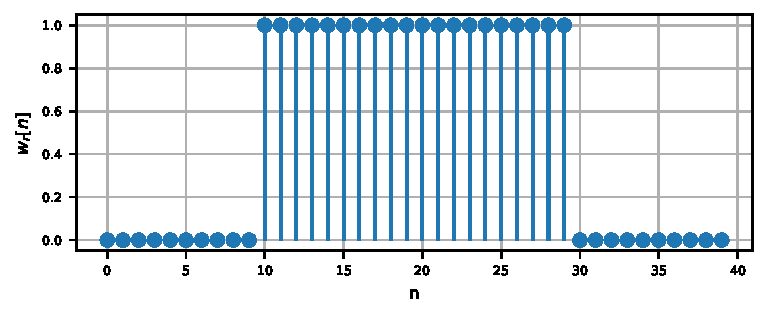
\includegraphics[width=.45\linewidth]{papers/sonogramm/images/rect_time.pdf}}
%     \qquad
%     \subfigure[Frequenzspektrum des Rechtecksfenster von Abbildung \ref{sonogramm:recttime}
%          mit einer Abtastfrequenz von 20 Hz. \label{sonogramm:rectfreq}]
%       {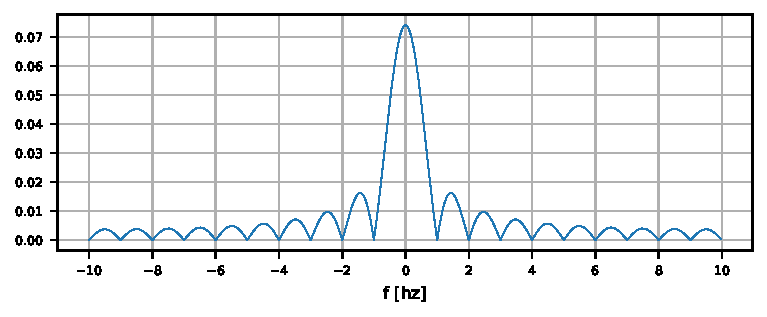
\includegraphics[
%         width=.45\linewidth
%         % scale = 1.2,
%         % trim = 0 40 0 0, clip,
%       ]{papers/sonogramm/images/rect_freq.pdf}}
%     \caption{
%         Frequenzanalyse eines Rechteckfensters. In (b)
%         sieht man die Nulldurchgänge bei vielfachen von $1/T$.
%     }
% \end{figure}
% \begin{figure}
%     \centering
%     \begin{subfigure}
%         \centering
%         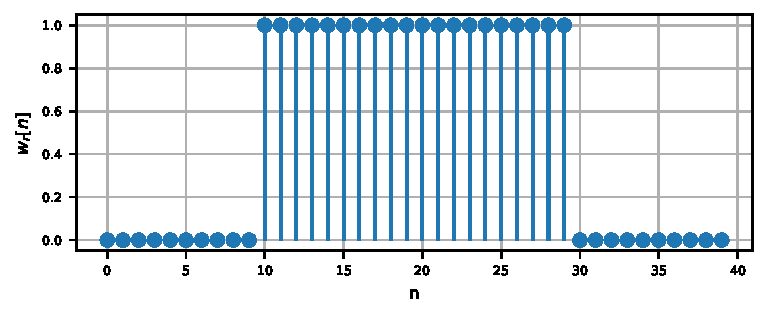
\includegraphics[width=1\linewidth]{papers/sonogramm/images/rect_time.pdf}
%         \caption{Rechtecksfenster mit $L_w = 20$ und T = 1 Sekunde.}
%         \label{sonogramm:recttime}
%     \end{subfigure}
%     \hfill
%     \begin{subfigure}
%         \centering
%         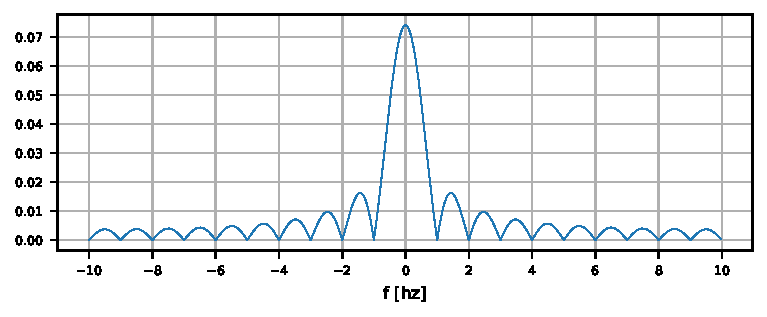
\includegraphics[width=1\linewidth]{papers/sonogramm/images/rect_freq.pdf}
%         \caption{Frequenzspektrum des Rechtecksfenster von Abbildung \ref{sonogramm:recttime}
%         mit einer Abtastfrequenz von 20 Hz.}
%         \label{sonogramm:rectfreq}
%     \end{subfigure}
%     \label{fig:three graphs}
%        \caption{Frequenzanalyse eines Rechteckfensters. In Abbildung \ref*{sonogramm:rectfreq}
%        sieht man die Nulldurchgänge bei vielfachen von $1/T$.}

% \end{figure}
\begin{figure}
    \centering
    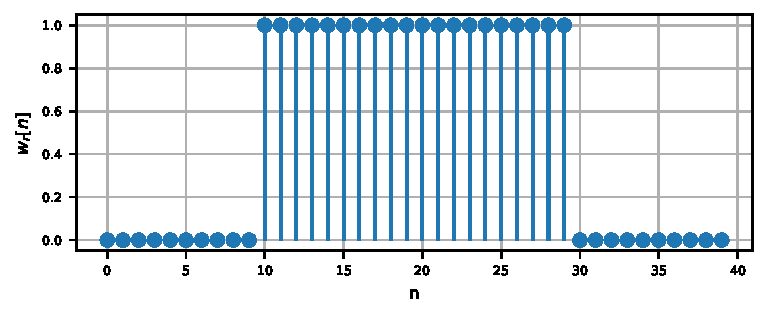
\includegraphics{papers/sonogramm/images/rect_time.pdf}
    \caption{Rechtecksfenster mit $L_w = 20$.
    \label{sonogramm:recttime}
    }
\end{figure}

\begin{figure}
    \centering
    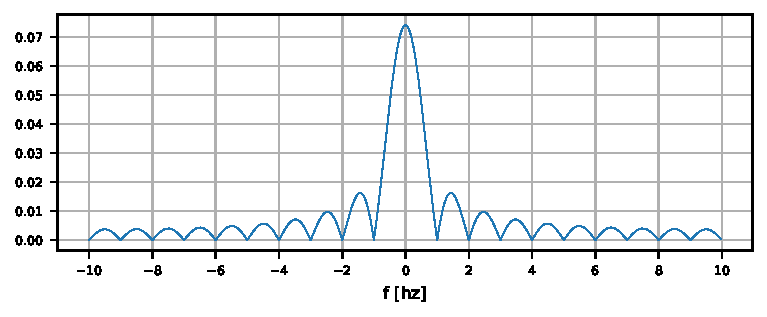
\includegraphics{papers/sonogramm/images/rect_freq.pdf}
    \caption{Frequenzspektrum des Rechtecksfenster von Abbildung \ref{sonogramm:recttime}
    mit einer Abtastfrequenz von 20 Hz. Die Nulldurchgänge sind jeweils bei ganzzahligen Vielfachen
    von $1/T$.
    \label{sonogramm:rectfreq}
    }
\end{figure}


\begin{figure}
    \centering
    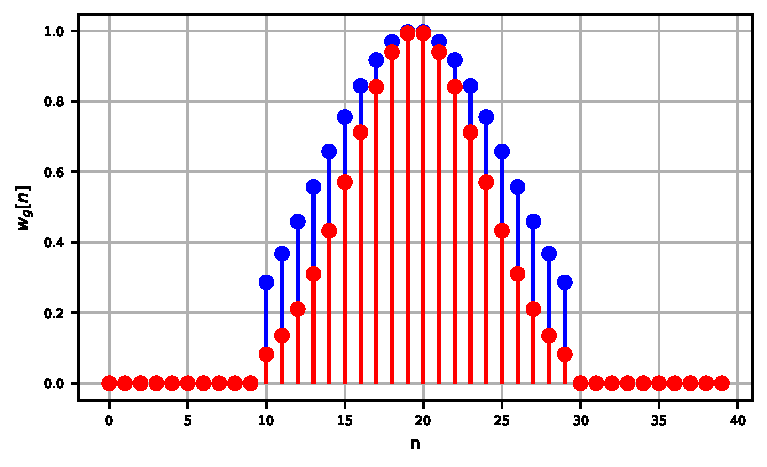
\includegraphics{papers/sonogramm/images/gauss_time.pdf}
    \caption{Gauss mit $L_w = 20$.
    \label{sonogramm:gausstime}
    }
\end{figure}

\begin{figure}
    \centering
    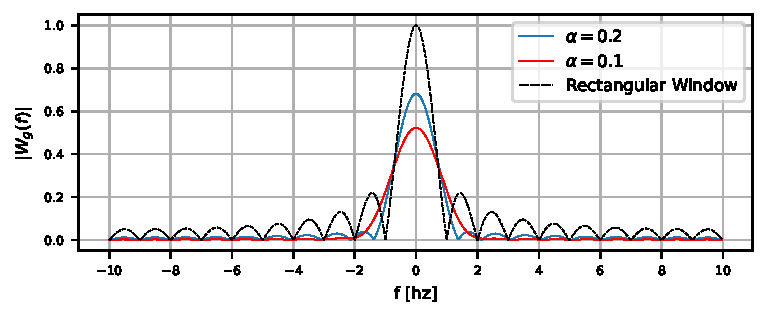
\includegraphics{papers/sonogramm/images/gauss_freq.pdf}
    \caption{Frequenzspektrum des Rechtecksfenster von Abbildung \ref{sonogramm:recttime}
    mit einer Abtastfrequenz von 20 Hz. Die Nulldurchgänge sind jeweils bei ganzzahligen Vielfachen
    von $1/T$.
    \label{sonogramm:gaussfreq}
    }
\end{figure}
TODO Grafik
